% Manuscript for the ISMB 2027 proceedings (Bioinformatics). OUP authoring template, contemporary large layout.
% Build with make (from paper/): numbers, tables and figures come from the result files.
\documentclass[webpdf,contemporary,large,namedate]{oup-authoring-template}

\usepackage{xspace}
\usepackage{booktabs}
\usepackage{xr-hyper}
% Supplementary references (S-<label>) are read from supplement.aux, so the supplement is built first (Makefile)
\externaldocument[S-]{supplement}
\usetikzlibrary{positioning,arrows.meta}
\definecolor{ink}{HTML}{0B0B0B}
\definecolor{ink2}{HTML}{52514E}
\definecolor{auditfill}{HTML}{FCEDE6}
\definecolor{gemfill}{HTML}{E9F1FB}
\graphicspath{{figures/}}


% no dotted rules above and below the abstract
\renewcommand{\dhorline}[3][0]{}

% every number in the paper comes from here (paper/scripts/make_numbers.py)
% Generated by paper/scripts/make_numbers.py. Do not edit by hand.
\newcommand{\NGenomes}{754\xspace}
\newcommand{\NSpecies}{669\xspace}
\newcommand{\NSlow}{58\xspace}
\newcommand{\NArchaea}{156\xspace}
\newcommand{\NInputs}{56\xspace}
\newcommand{\NLiterature}{8\xspace}
\newcommand{\NGenomeExtension}{161\xspace}
\newcommand{\NOriginal}{294\xspace}
\newcommand{\NMadinExtension}{291\xspace}
\newcommand{\NExcluded}{10\xspace}
\newcommand{\NExcludedKevbrina}{4\xspace}
\newcommand{\NExcludedWord}{ten\xspace}
\newcommand{\NExcludedKevbrinaWord}{four\xspace}
\newcommand{\NExcludedSourcesWord}{five\xspace}
\newcommand{\NLiteratureWord}{eight\xspace}
\newcommand{\ErrSameGenus}{1.75\xspace}
\newcommand{\RhoSameGenus}{0.74\xspace}
\newcommand{\AucSameGenus}{0.85\xspace}
\newcommand{\ErrRefSameGenus}{1.73\xspace}
\newcommand{\RhoRefSameGenus}{0.84\xspace}
\newcommand{\TempMAESameGenus}{5.0\xspace}
\newcommand{\RhoTempSameGenus}{0.86\xspace}
\newcommand{\FixedErrSameGenus}{1.82\xspace}
\newcommand{\CoarseErrSameGenus}{1.75\xspace}
\newcommand{\FixedErrRefSameGenus}{1.75\xspace}
\newcommand{\ErrNewGenus}{1.91\xspace}
\newcommand{\RhoNewGenus}{0.71\xspace}
\newcommand{\AucNewGenus}{0.84\xspace}
\newcommand{\ErrRefNewGenus}{1.81\xspace}
\newcommand{\RhoRefNewGenus}{0.83\xspace}
\newcommand{\TempMAENewGenus}{5.7\xspace}
\newcommand{\RhoTempNewGenus}{0.83\xspace}
\newcommand{\FixedErrNewGenus}{1.96\xspace}
\newcommand{\CoarseErrNewGenus}{1.92\xspace}
\newcommand{\FixedErrRefNewGenus}{1.79\xspace}
\newcommand{\ErrNewFamily}{2.06\xspace}
\newcommand{\RhoNewFamily}{0.66\xspace}
\newcommand{\AucNewFamily}{0.81\xspace}
\newcommand{\ErrRefNewFamily}{1.91\xspace}
\newcommand{\RhoRefNewFamily}{0.81\xspace}
\newcommand{\TempMAENewFamily}{5.8\xspace}
\newcommand{\RhoTempNewFamily}{0.83\xspace}
\newcommand{\FixedErrNewFamily}{2.07\xspace}
\newcommand{\CoarseErrNewFamily}{2.07\xspace}
\newcommand{\FixedErrRefNewFamily}{1.88\xspace}
\newcommand{\ErrNewOrder}{2.08\xspace}
\newcommand{\RhoNewOrder}{0.66\xspace}
\newcommand{\AucNewOrder}{0.82\xspace}
\newcommand{\ErrRefNewOrder}{1.93\xspace}
\newcommand{\RhoRefNewOrder}{0.81\xspace}
\newcommand{\TempMAENewOrder}{6.0\xspace}
\newcommand{\RhoTempNewOrder}{0.81\xspace}
\newcommand{\FixedErrNewOrder}{2.08\xspace}
\newcommand{\CoarseErrNewOrder}{2.08\xspace}
\newcommand{\FixedErrRefNewOrder}{1.91\xspace}
\newcommand{\NSeedsHeadline}{3\xspace}
\newcommand{\NHeadlineRows}{742\xspace}
\newcommand{\SlowCalledSpecies}{9\xspace}
\newcommand{\SlowCalledTrueSpecies}{8\xspace}
\newcommand{\SlowTotalSpecies}{52\xspace}
\newcommand{\SlowCalledOrder}{0\xspace}
\newcommand{\SlowCalledTrueOrder}{0\xspace}
\newcommand{\SlowTotalOrder}{52\xspace}
\newcommand{\CoverSameGenus}{80\xspace}
\newcommand{\CoverNewGenus}{80\xspace}
\newcommand{\CoverNewFamily}{80\xspace}
\newcommand{\CoverNewOrder}{81\xspace}
\newcommand{\CoverRefMin}{79\xspace}
\newcommand{\CoverRefMax}{80\xspace}
\newcommand{\CoverTempMin}{81\xspace}
\newcommand{\CoverTempMax}{84\xspace}
\newcommand{\NGEMPredicted}{9,139\xspace}
\newcommand{\GEMShareSameGenus}{11\xspace}
\newcommand{\GEMShareNewGenus}{24\xspace}
\newcommand{\GEMShareNewFamily}{27\xspace}
\newcommand{\GEMShareNewOrder}{38\xspace}
\newcommand{\GEMShareNoGenus}{89\xspace}
\newcommand{\GEMMedianHours}{2.8\xspace}
\newcommand{\GEMShareSlow}{0.4\xspace}
\newcommand{\GEMNSlow}{39\xspace}
\newcommand{\GEMSlowTopOrder}{Anaerolineales\xspace}
\newcommand{\GEMSlowTopOrderN}{21\xspace}
\newcommand{\GEMMedianHuman}{1.6\xspace}
\newcommand{\GEMNHuman}{3,747\xspace}
\newcommand{\GEMNewOrderHuman}{26\xspace}
\newcommand{\GEMMedianAquatic}{6.7\xspace}
\newcommand{\GEMNAquatic}{2,522\xspace}
\newcommand{\GEMNewOrderAquatic}{58\xspace}
\newcommand{\GEMMedianBuilt}{1.0\xspace}
\newcommand{\GEMNBuilt}{915\xspace}
\newcommand{\GEMNewOrderBuilt}{10\xspace}
\newcommand{\GEMMedianTerrestrial}{7.3\xspace}
\newcommand{\GEMNTerrestrial}{497\xspace}
\newcommand{\GEMNewOrderTerrestrial}{55\xspace}
\newcommand{\GEMMedianWastewater}{7.1\xspace}
\newcommand{\GEMNWastewater}{492\xspace}
\newcommand{\GEMNewOrderWastewater}{60\xspace}
\newcommand{\GEMSlowSecondOrder}{Nitrososphaerales\xspace}
\newcommand{\GEMSlowSecondOrderN}{13\xspace}
\newcommand{\RelOursErr}{1.76\xspace}
\newcommand{\RelOursRho}{0.72\xspace}
\newcommand{\RelOursAuc}{0.85\xspace}
\newcommand{\RelOursTempErr}{1.70\xspace}
\newcommand{\RelOursTempRho}{0.76\xspace}
\newcommand{\RelOursTempAuc}{0.87\xspace}
\newcommand{\RelGRodonErr}{1.92\xspace}
\newcommand{\RelGRodonRho}{0.73\xspace}
\newcommand{\RelGRodonAuc}{0.84\xspace}
\newcommand{\RelGRodonNoTempErr}{2.40\xspace}
\newcommand{\RelGRodonNoTempRho}{0.52\xspace}
\newcommand{\RelGRodonNoTempAuc}{0.75\xspace}
\newcommand{\RelPhydonErr}{1.85\xspace}
\newcommand{\RelPhydonRho}{0.70\xspace}
\newcommand{\RelPhydonAuc}{0.81\xspace}
\newcommand{\RelN}{680\xspace}
\newcommand{\RelNPhydon}{665\xspace}
\newcommand{\RelNSeeds}{3\xspace}
\newcommand{\RelOursTempBeatsPhydon}{3\xspace}
\newcommand{\RelOursTempBeatsGRodon}{3\xspace}
\newcommand{\RelOursBeatsPhydon}{3\xspace}
\newcommand{\RelOursBeatsGRodon}{3\xspace}
\newcommand{\PosCtrlCaughtWord}{eight\xspace}
\newcommand{\PosCtrlNWord}{nine\xspace}
\newcommand{\KevFoldWith}{5.2\xspace}
\newcommand{\KevLowWith}{2.1\xspace}
\newcommand{\KevHighWith}{12.7\xspace}
\newcommand{\KevPWith}{0.01\xspace}
\newcommand{\KevNWith}{11\xspace}
\newcommand{\KevFoldWithout}{1.5\xspace}
\newcommand{\KevLowWithout}{0.5\xspace}
\newcommand{\KevHighWithout}{4.8\xspace}
\newcommand{\KevPWithout}{0.90\xspace}
\newcommand{\KevNWithout}{7\xspace}
\newcommand{\KevLabelMin}{112\xspace}
\newcommand{\KevLabelMax}{187\xspace}
\newcommand{\KevRecordMin}{2,717\xspace}
\newcommand{\KevRecordMax}{4,576\xspace}
\newcommand{\KevRatio}{24\xspace}
\newcommand{\NStudiesCompared}{27\xspace}
\newcommand{\NStudiesFlagged}{8\xspace}
\newcommand{\SixteenOwnDist}{0.036\xspace}
\newcommand{\SixteenNearDist}{0.158\xspace}
\newcommand{\SixteenN}{540\xspace}
\newcommand{\SixteenFarther}{65\xspace}
\newcommand{\SixteenShift}{0.09\xspace}
\newcommand{\SixteenNGenomeCopy}{685\xspace}
\newcommand{\SixteenErrNcbiSpecies}{1.76\xspace}
\newcommand{\SixteenErrGenomeSpecies}{1.75\xspace}
\newcommand{\SixteenErrMixedSpecies}{1.79\xspace}
\newcommand{\SixteenMixedWorseSpecies}{3\xspace}
\newcommand{\SixteenErrNcbiOrder}{1.98\xspace}
\newcommand{\SixteenErrGenomeOrder}{1.97\xspace}
\newcommand{\SixteenErrMixedOrder}{2.03\xspace}
\newcommand{\SixteenMixedWorseOrder}{3\xspace}
\newcommand{\SixteenNSeeds}{3\xspace}
\newcommand{\NSeedsAblation}{10\xspace}
\newcommand{\AblFinalErrSpecies}{1.82\xspace}
\newcommand{\AblFinalRhoSpecies}{0.74\xspace}
\newcommand{\AblFinalAucSpecies}{0.84\xspace}
\newcommand{\AblGStatErrSpecies}{1.93\xspace}
\newcommand{\AblGStatRhoSpecies}{0.70\xspace}
\newcommand{\AblGStatAucSpecies}{0.83\xspace}
\newcommand{\AblGStatWorseSpecies}{10\xspace}
\newcommand{\AblLifeErrSpecies}{1.82\xspace}
\newcommand{\AblLifeRhoSpecies}{0.74\xspace}
\newcommand{\AblLifeAucSpecies}{0.84\xspace}
\newcommand{\AblLifeWorseSpecies}{6\xspace}
\newcommand{\AblGenesErrSpecies}{2.09\xspace}
\newcommand{\AblGenesRhoSpecies}{0.66\xspace}
\newcommand{\AblGenesAucSpecies}{0.81\xspace}
\newcommand{\AblGenesWorseSpecies}{10\xspace}
\newcommand{\AblSixteenErrSpecies}{1.82\xspace}
\newcommand{\AblSixteenRhoSpecies}{0.74\xspace}
\newcommand{\AblSixteenAucSpecies}{0.84\xspace}
\newcommand{\AblSixteenWorseSpecies}{3\xspace}
\newcommand{\AblPhyloErrSpecies}{1.84\xspace}
\newcommand{\AblPhyloRhoSpecies}{0.73\xspace}
\newcommand{\AblPhyloAucSpecies}{0.84\xspace}
\newcommand{\AblPhyloWorseSpecies}{9\xspace}
\newcommand{\AblAddedErrSpecies}{1.86\xspace}
\newcommand{\AblAddedRhoSpecies}{0.73\xspace}
\newcommand{\AblAddedAucSpecies}{0.84\xspace}
\newcommand{\AblAddedWorseSpecies}{10\xspace}
\newcommand{\AblEnergyErrSpecies}{1.82\xspace}
\newcommand{\AblEnergyRhoSpecies}{0.74\xspace}
\newcommand{\AblEnergyAucSpecies}{0.84\xspace}
\newcommand{\AblEnergyWorseSpecies}{6\xspace}
\newcommand{\AblPredTempErrSpecies}{1.80\xspace}
\newcommand{\AblPredTempRhoSpecies}{0.74\xspace}
\newcommand{\AblPredTempAucSpecies}{0.84\xspace}
\newcommand{\AblPredTempWorseSpecies}{4\xspace}
\newcommand{\AblFinalErrOrder}{2.09\xspace}
\newcommand{\AblFinalRhoOrder}{0.65\xspace}
\newcommand{\AblFinalAucOrder}{0.80\xspace}
\newcommand{\AblGStatErrOrder}{2.39\xspace}
\newcommand{\AblGStatRhoOrder}{0.57\xspace}
\newcommand{\AblGStatAucOrder}{0.76\xspace}
\newcommand{\AblGStatWorseOrder}{10\xspace}
\newcommand{\AblLifeErrOrder}{2.07\xspace}
\newcommand{\AblLifeRhoOrder}{0.66\xspace}
\newcommand{\AblLifeAucOrder}{0.81\xspace}
\newcommand{\AblLifeWorseOrder}{4\xspace}
\newcommand{\AblGenesErrOrder}{2.64\xspace}
\newcommand{\AblGenesRhoOrder}{0.46\xspace}
\newcommand{\AblGenesAucOrder}{0.73\xspace}
\newcommand{\AblGenesWorseOrder}{10\xspace}
\newcommand{\AblSixteenErrOrder}{2.09\xspace}
\newcommand{\AblSixteenRhoOrder}{0.65\xspace}
\newcommand{\AblSixteenAucOrder}{0.79\xspace}
\newcommand{\AblSixteenWorseOrder}{4\xspace}
\newcommand{\AblPhyloErrOrder}{2.07\xspace}
\newcommand{\AblPhyloRhoOrder}{0.66\xspace}
\newcommand{\AblPhyloAucOrder}{0.81\xspace}
\newcommand{\AblPhyloWorseOrder}{2\xspace}
\newcommand{\AblAddedErrOrder}{2.13\xspace}
\newcommand{\AblAddedRhoOrder}{0.65\xspace}
\newcommand{\AblAddedAucOrder}{0.80\xspace}
\newcommand{\AblAddedWorseOrder}{10\xspace}
\newcommand{\AblEnergyErrOrder}{2.11\xspace}
\newcommand{\AblEnergyRhoOrder}{0.65\xspace}
\newcommand{\AblEnergyAucOrder}{0.80\xspace}
\newcommand{\AblEnergyWorseOrder}{7\xspace}
\newcommand{\AblPredTempErrOrder}{2.08\xspace}
\newcommand{\AblPredTempRhoOrder}{0.66\xspace}
\newcommand{\AblPredTempAucOrder}{0.80\xspace}
\newcommand{\AblPredTempWorseOrder}{2\xspace}
\newcommand{\TuneErrBefore}{2.14\xspace}
\newcommand{\TuneErrAfter}{2.13\xspace}
\newcommand{\TuneRhoBefore}{0.63\xspace}
\newcommand{\TuneRhoAfter}{0.65\xspace}
\newcommand{\TuneAucBefore}{0.79\xspace}
\newcommand{\TuneAucAfter}{0.80\xspace}
\newcommand{\TuneBetter}{4\xspace}
\newcommand{\TuneNSeeds}{5\xspace}
\newcommand{\MagErr}{1.86\xspace}
\newcommand{\MagIsoErr}{1.70\xspace}
\newcommand{\MagNSpecies}{47\xspace}
\newcommand{\MagNGenomes}{717\xspace}
\newcommand{\MagGap}{1.08\xspace}
\newcommand{\MagGapMax}{2.2\xspace}
\newcommand{\MagGapSmaller}{41\xspace}
\newcommand{\IndepErr}{2.09\xspace}
\newcommand{\IndepN}{294\xspace}
\newcommand{\BaseRelErrSameGenus}{1.81\xspace}
\newcommand{\BaseRelRhoSameGenus}{0.66\xspace}
\newcommand{\BaseRelAucSameGenus}{0.80\xspace}
\newcommand{\BaseMedErrSameGenus}{2.72\xspace}
\newcommand{\CIErrLoSameGenus}{1.67\xspace}
\newcommand{\CIErrHiSameGenus}{1.86\xspace}
\newcommand{\CIRhoLoSameGenus}{0.68\xspace}
\newcommand{\CIRhoHiSameGenus}{0.78\xspace}
\newcommand{\CIDiffLoSameGenus}{$-$0.21\xspace}
\newcommand{\CIDiffHiSameGenus}{0.05\xspace}
\newcommand{\BaseRelErrNewGenus}{2.12\xspace}
\newcommand{\BaseRelRhoNewGenus}{0.57\xspace}
\newcommand{\BaseRelAucNewGenus}{0.79\xspace}
\newcommand{\BaseMedErrNewGenus}{2.74\xspace}
\newcommand{\CIErrLoNewGenus}{1.81\xspace}
\newcommand{\CIErrHiNewGenus}{2.02\xspace}
\newcommand{\CIRhoLoNewGenus}{0.66\xspace}
\newcommand{\CIRhoHiNewGenus}{0.76\xspace}
\newcommand{\CIDiffLoNewGenus}{$-$0.42\xspace}
\newcommand{\CIDiffHiNewGenus}{$-$0.02\xspace}
\newcommand{\BaseRelErrNewFamily}{2.59\xspace}
\newcommand{\BaseRelRhoNewFamily}{0.40\xspace}
\newcommand{\BaseRelAucNewFamily}{0.72\xspace}
\newcommand{\BaseMedErrNewFamily}{2.86\xspace}
\newcommand{\CIErrLoNewFamily}{1.93\xspace}
\newcommand{\CIErrHiNewFamily}{2.24\xspace}
\newcommand{\CIRhoLoNewFamily}{0.59\xspace}
\newcommand{\CIRhoHiNewFamily}{0.72\xspace}
\newcommand{\CIDiffLoNewFamily}{$-$0.84\xspace}
\newcommand{\CIDiffHiNewFamily}{$-$0.21\xspace}
\newcommand{\BaseRelErrNewOrder}{2.45\xspace}
\newcommand{\BaseRelRhoNewOrder}{0.41\xspace}
\newcommand{\BaseRelAucNewOrder}{0.72\xspace}
\newcommand{\BaseMedErrNewOrder}{2.78\xspace}
\newcommand{\CIErrLoNewOrder}{1.96\xspace}
\newcommand{\CIErrHiNewOrder}{2.23\xspace}
\newcommand{\CIRhoLoNewOrder}{0.57\xspace}
\newcommand{\CIRhoHiNewOrder}{0.72\xspace}
\newcommand{\CIDiffLoNewOrder}{$-$0.74\xspace}
\newcommand{\CIDiffHiNewOrder}{$-$0.16\xspace}
\newcommand{\ShuffleErrSpecies}{2.91\xspace}
\newcommand{\ShuffleRhoSpecies}{0.00\xspace}
\newcommand{\ShuffleMedErrSpecies}{2.73\xspace}
\newcommand{\ShuffleErrOrder}{2.89\xspace}
\newcommand{\ShuffleRhoOrder}{$-$0.04\xspace}
\newcommand{\ShuffleMedErrOrder}{2.72\xspace}
\newcommand{\PairGRodonN}{680\xspace}
\newcommand{\PairGRodonBetter}{349\xspace}
\newcommand{\PairGRodonP}{0.07\xspace}
\newcommand{\PairGRodonDiffLo}{$-$0.26\xspace}
\newcommand{\PairGRodonDiffHi}{$-$0.04\xspace}
\newcommand{\PairTempGRodonN}{680\xspace}
\newcommand{\PairTempGRodonBetter}{383\xspace}
\newcommand{\PairTempGRodonP}{$1.5\times10^{-6}$\xspace}
\newcommand{\PairPhydonN}{665\xspace}
\newcommand{\PairPhydonBetter}{347\xspace}
\newcommand{\PairPhydonP}{0.11\xspace}
\newcommand{\PairPhydonDiffLo}{$-$0.26\xspace}
\newcommand{\PairPhydonDiffHi}{0.05\xspace}
\newcommand{\PairTempPhydonN}{665\xspace}
\newcommand{\PairTempPhydonBetter}{355\xspace}
\newcommand{\PairTempPhydonP}{$3.9\times10^{-4}$\xspace}
\newcommand{\CIMagErrLo}{1.60\xspace}
\newcommand{\CIMagErrHi}{2.20\xspace}
\newcommand{\CIMagDiffLo}{$-$0.16\xspace}
\newcommand{\CIMagDiffHi}{0.32\xspace}
\newcommand{\CovNovAllSpecies}{80\xspace}
\newcommand{\CovNovArchSpecies}{79\xspace}
\newcommand{\CovNovSlowSpecies}{44\xspace}
\newcommand{\CovNovFastSpecies}{83\xspace}
\newcommand{\CovDomAllSpecies}{80\xspace}
\newcommand{\CovDomArchSpecies}{79\xspace}
\newcommand{\CovDomSlowSpecies}{45\xspace}
\newcommand{\CovDomFastSpecies}{83\xspace}
\newcommand{\CovNovAllOrder}{80\xspace}
\newcommand{\CovNovArchOrder}{73\xspace}
\newcommand{\CovNovSlowOrder}{26\xspace}
\newcommand{\CovNovFastOrder}{85\xspace}
\newcommand{\CovDomAllOrder}{79\xspace}
\newcommand{\CovDomArchOrder}{78\xspace}
\newcommand{\CovDomSlowOrder}{29\xspace}
\newcommand{\CovDomFastOrder}{83\xspace}
\newcommand{\CovDomArchMin}{78\xspace}
\newcommand{\CovDomSlowMin}{29\xspace}
\newcommand{\CovDomSlowMax}{45\xspace}
\newcommand{\SlowProbAucSpecies}{0.84\xspace}
\newcommand{\SlowProbTopSpecies}{24\xspace}
\newcommand{\SlowProbBrierSpecies}{0.057\xspace}
\newcommand{\SlowProbBrierBaseSpecies}{0.072\xspace}
\newcommand{\SlowProbAucOrder}{0.81\xspace}
\newcommand{\SlowProbTopOrder}{22\xspace}
\newcommand{\SlowProbBrierOrder}{0.065\xspace}
\newcommand{\SlowProbBrierBaseOrder}{0.072\xspace}
\newcommand{\SlowProbECEMax}{0.012\xspace}
\newcommand{\SlowBaseRate}{8\xspace}
\newcommand{\ErrSlowSpecies}{4.5\xspace}
\newcommand{\ErrArchSpecies}{1.87\xspace}
\newcommand{\ErrBactSpecies}{1.72\xspace}
\newcommand{\ErrSlowOrder}{6.3\xspace}
\newcommand{\ErrArchOrder}{2.43\xspace}
\newcommand{\ErrBactOrder}{2.02\xspace}
\newcommand{\GEMNArchaea}{183\xspace}
\newcommand{\EsmN}{742\xspace}
\newcommand{\EsmFeatErrSameGenus}{1.82\xspace}
\newcommand{\EsmFeatRhoSameGenus}{0.74\xspace}
\newcommand{\EsmProbeErrSameGenus}{1.86\xspace}
\newcommand{\EsmProbeRhoSameGenus}{0.75\xspace}
\newcommand{\EsmTreesErrSameGenus}{2.03\xspace}
\newcommand{\EsmTreesRhoSameGenus}{0.71\xspace}
\newcommand{\EsmCombErrSameGenus}{1.78\xspace}
\newcommand{\EsmCombRhoSameGenus}{0.76\xspace}
\newcommand{\EsmFeatErrNewGenus}{1.96\xspace}
\newcommand{\EsmFeatRhoNewGenus}{0.71\xspace}
\newcommand{\EsmProbeErrNewGenus}{1.90\xspace}
\newcommand{\EsmProbeRhoNewGenus}{0.73\xspace}
\newcommand{\EsmTreesErrNewGenus}{2.11\xspace}
\newcommand{\EsmTreesRhoNewGenus}{0.67\xspace}
\newcommand{\EsmCombErrNewGenus}{1.91\xspace}
\newcommand{\EsmCombRhoNewGenus}{0.74\xspace}
\newcommand{\EsmFeatErrNewFamily}{2.07\xspace}
\newcommand{\EsmFeatRhoNewFamily}{0.67\xspace}
\newcommand{\EsmProbeErrNewFamily}{2.00\xspace}
\newcommand{\EsmProbeRhoNewFamily}{0.69\xspace}
\newcommand{\EsmTreesErrNewFamily}{2.19\xspace}
\newcommand{\EsmTreesRhoNewFamily}{0.62\xspace}
\newcommand{\EsmCombErrNewFamily}{2.03\xspace}
\newcommand{\EsmCombRhoNewFamily}{0.70\xspace}
\newcommand{\EsmFeatErrNewOrder}{2.08\xspace}
\newcommand{\EsmFeatRhoNewOrder}{0.67\xspace}
\newcommand{\EsmProbeErrNewOrder}{2.02\xspace}
\newcommand{\EsmProbeRhoNewOrder}{0.68\xspace}
\newcommand{\EsmTreesErrNewOrder}{2.23\xspace}
\newcommand{\EsmTreesRhoNewOrder}{0.61\xspace}
\newcommand{\EsmCombErrNewOrder}{2.05\xspace}
\newcommand{\EsmCombRhoNewOrder}{0.70\xspace}
\newcommand{\EsmProbePSameGenus}{0.87\xspace}
\newcommand{\EsmProbeBetterSameGenus}{368\xspace}
\newcommand{\EsmCombPSameGenus}{$3.1\times10^{-4}$\xspace}
\newcommand{\EsmCombBetterSameGenus}{426\xspace}
\newcommand{\EsmPairNSameGenus}{741\xspace}
\newcommand{\EsmProbePNewOrder}{0.99\xspace}
\newcommand{\EsmProbeBetterNewOrder}{357\xspace}
\newcommand{\EsmCombPNewOrder}{$6.1\times10^{-5}$\xspace}
\newcommand{\EsmCombBetterNewOrder}{423\xspace}
\newcommand{\EsmPairNNewOrder}{741\xspace}
\newcommand{\TenNSeeds}{10\xspace}
\newcommand{\TenModelErrSpecies}{1.82\xspace}
\newcommand{\TenBaseErrSpecies}{1.79\xspace}
\newcommand{\TenModelRhoSpecies}{0.74\xspace}
\newcommand{\TenBaseRhoSpecies}{0.67\xspace}
\newcommand{\TenModelWinsSpecies}{3\xspace}
\newcommand{\TenPGenomeSpecies}{0.02\xspace}
\newcommand{\TenModelWinsDeepMin}{10\xspace}
\newcommand{\TenPGenomeDeepMax}{$<$\,10$^{-4}$\xspace}
\newcommand{\RefitErrSpecies}{1.85\xspace}
\newcommand{\RefitFullErrSpecies}{1.82\xspace}
\newcommand{\FlagErrSpecies}{1.79\xspace}
\newcommand{\FlagFullErrSpecies}{1.81\xspace}
\newcommand{\RefitErrOrder}{2.10\xspace}
\newcommand{\RefitFullErrOrder}{2.08\xspace}
\newcommand{\FlagErrOrder}{2.02\xspace}
\newcommand{\FlagFullErrOrder}{2.05\xspace}
\newcommand{\RefitMaxDiff}{0.03\xspace}
\newcommand{\FlagNLabels}{25\xspace}
\newcommand{\DupMaxChange}{0.005\xspace}
\newcommand{\RelOrdOursErr}{2.08\xspace}
\newcommand{\RelOrdOursRho}{0.64\xspace}
\newcommand{\RelOrdOursAuc}{0.82\xspace}
\newcommand{\RelOrdOursTempErr}{1.96\xspace}
\newcommand{\RelOrdOursTempRho}{0.70\xspace}
\newcommand{\RelOrdOursTempAuc}{0.83\xspace}
\newcommand{\RelOrdGRodonErr}{1.92\xspace}
\newcommand{\RelOrdGRodonRho}{0.73\xspace}
\newcommand{\RelOrdGRodonAuc}{0.84\xspace}
\newcommand{\RelOrdGRodonNoTempErr}{2.40\xspace}
\newcommand{\RelOrdGRodonNoTempRho}{0.52\xspace}
\newcommand{\RelOrdGRodonNoTempAuc}{0.75\xspace}
\newcommand{\RelOrdPhydonErr}{2.84\xspace}
\newcommand{\RelOrdPhydonRho}{0.58\xspace}
\newcommand{\RelOrdPhydonAuc}{0.76\xspace}
\newcommand{\PairOrdGRodonN}{680\xspace}
\newcommand{\PairOrdGRodonBetter}{330\xspace}
\newcommand{\PairOrdGRodonP}{0.007\xspace}
\newcommand{\PairOrdPhydonN}{665\xspace}
\newcommand{\PairOrdPhydonBetter}{433\xspace}
\newcommand{\PairOrdPhydonP}{$<$\,10$^{-4}$\xspace}
\newcommand{\PairOrdGRodonNoTempN}{680\xspace}
\newcommand{\PairOrdGRodonNoTempBetter}{406\xspace}
\newcommand{\PairOrdGRodonNoTempP}{$<$\,10$^{-4}$\xspace}
\newcommand{\PairOrdTempGRodonN}{680\xspace}
\newcommand{\PairOrdTempGRodonBetter}{351\xspace}
\newcommand{\PairOrdTempGRodonP}{0.96\xspace}
\newcommand{\ExtNCurated}{51\xspace}
\newcommand{\NSeedsExternal}{5\xspace}
\newcommand{\PhydonOrderMapped}{99.6\xspace}
\newcommand{\ExtNSources}{51\xspace}
\newcommand{\ExtN}{48\xspace}
\newcommand{\ExtNSlow}{7\xspace}
\newcommand{\ExtNArchaea}{3\xspace}
\newcommand{\ExtNSameGenus}{7\xspace}
\newcommand{\ExtNNewGenus}{18\xspace}
\newcommand{\ExtNNewFamily}{9\xspace}
\newcommand{\ExtNNewOrder}{14\xspace}
\newcommand{\ExtModelErr}{2.53\xspace}
\newcommand{\ExtModelLo}{1.91\xspace}
\newcommand{\ExtModelHi}{3.30\xspace}
\newcommand{\ExtModelRho}{0.62\xspace}
\newcommand{\ExtBaseErr}{3.65\xspace}
\newcommand{\ExtBaseLo}{2.35\xspace}
\newcommand{\ExtBaseHi}{4.95\xspace}
\newcommand{\ExtBaseRho}{0.34\xspace}
\newcommand{\ExtGRodonErr}{3.42\xspace}
\newcommand{\ExtGRodonLo}{2.64\xspace}
\newcommand{\ExtGRodonHi}{4.72\xspace}
\newcommand{\ExtGRodonRho}{0.34\xspace}
\newcommand{\ExtModelErrSameGenus}{1.15\xspace}
\newcommand{\ExtBaseErrSameGenus}{1.57\xspace}
\newcommand{\ExtModelErrNewGenus}{2.42\xspace}
\newcommand{\ExtBaseErrNewGenus}{3.63\xspace}
\newcommand{\ExtModelErrNewFamily}{2.71\xspace}
\newcommand{\ExtBaseErrNewFamily}{3.64\xspace}
\newcommand{\ExtModelErrNewOrder}{4.69\xspace}
\newcommand{\ExtBaseErrNewOrder}{5.33\xspace}
\newcommand{\ExtBetterBase}{32\xspace}
\newcommand{\ExtPBase}{0.007\xspace}
\newcommand{\ExtBetterGRodon}{34\xspace}
\newcommand{\ExtPGRodon}{0.001\xspace}
\newcommand{\ExtCoverage}{67\xspace}
\newcommand{\ExtCoverageP}{0.03\xspace}
\newcommand{\ExtCoverageSlowIn}{1\xspace}
\newcommand{\ExtSlowAuc}{0.92\xspace}
\newcommand{\ExtBias}{1.16\xspace}
\newcommand{\PglsLambda}{0.73\xspace}
\newcommand{\PglsNGroups}{592\xspace}
\newcommand{\PglsRegFold}{0.80\xspace}
\newcommand{\PglsRegP}{0.042\xspace}
\newcommand{\PglsEnergyMinP}{0.34\xspace}
\newcommand{\SlowTransporterOR}{0.27\xspace}
\newcommand{\SlowTransporterP}{$9.4\times10^{-5}$\xspace}
\newcommand{\KmerK}{6\xspace}
\newcommand{\EaKJ}{65\xspace}
\newcommand{\TRefC}{20\xspace}
\newcommand{\NLandmarks}{16\xspace}
\newcommand{\MinContig}{200\xspace}
\newcommand{\MinTrainKb}{100\xspace}
\newcommand{\MinRibosomal}{10\xspace}
\newcommand{\NRibosomalFamilies}{75\xspace}
\newcommand{\NLifestyleFamilies}{34\xspace}
\newcommand{\NLifestyleFeatures}{14\xspace}
\newcommand{\NEnergyFamilies}{27\xspace}
\newcommand{\NEnergyFeatures}{15\xspace}
\newcommand{\NGRodonFeatures}{4\xspace}
\newcommand{\NGRodonFeaturesWord}{four\xspace}
\newcommand{\DriftSD}{3\xspace}
\newcommand{\NSeedsTable}{3\xspace}
\newcommand{\NSeedsMag}{5\xspace}
\newcommand{\GTDBRelease}{232\xspace}
\newcommand{\NGrowthTable}{928\xspace}
\newcommand{\NGEMTotal}{52,515\xspace}
\newcommand{\NGEMHQ}{9,143\xspace}
\newcommand{\ScreenFoldWord}{five\xspace}
\newcommand{\StudyFoldWord}{three\xspace}
\newcommand{\StudyFold}{3\xspace}
\newcommand{\NBootDraws}{2,000\xspace}
\newcommand{\TraceTolPct}{2\xspace}
\newcommand{\KEigen}{20\xspace}
\newcommand{\NForestTrees}{300\xspace}
\newcommand{\EsmNRibosomal}{60\xspace}
\newcommand{\EsmNOther}{100\xspace}
\newcommand{\EsmPCTrees}{64\xspace}
\newcommand{\EsmPCComb}{32\xspace}
\newcommand{\NTuneCandidates}{20\xspace}
\newcommand{\NTuneShuffles}{3\xspace}
\newcommand{\NTuneFolds}{3\xspace}
\newcommand{\NFolds}{5\xspace}
\newcommand{\SynKnownWord}{six\xspace}
\newcommand{\SynFoundWord}{three\xspace}
\newcommand{\SynFalse}{66\xspace}

\xspaceaddexceptions{\%}

\begin{document}

\journaltitle{Bioinformatics}
\pubyear{2027}
\copyrightyear{2027}
\firstpage{1}

\title[How fast do uncultured microbes grow?]{How fast do uncultured microbes grow?}

% anonymized for review
\author{Anonymous Authors}

\abstract{\rmfamily\fontseries{m}\selectfont\textbf{Motivation:} Most microbes are known only from genomes assembled out of
environmental DNA, so how fast they grow has to be read from those genomes. Most such genomes have no close relative with a
measured growth rate, and none comes with the measured growth temperature that current predictors need.\\
\textbf{Results:} We predict the maximal doubling time, the growth temperature and a temperature-standardized doubling time
from the genome alone, and test every prediction with whole lineages held out. Predictions are typically within
\ErrSameGenus-fold with a labeled relative in the same genus, and within \ErrNewOrder-fold with none in
the same order. Metagenome-assembled genomes give much the same predictions as isolates. Without the measured temperature,
the model is as accurate as gRodon and Phydon given it for new species (\RelOursErr- against \RelGRodonErr- and
\RelPhydonErr-fold) but trails gRodon given it for new orders. On \ExtN species absent from both training compilations it is
off by \ExtModelErr-fold, against \ExtBaseErr-fold from taxonomy alone.
Auditing the training labels, we found \NExcludedKevbrinaWord values from one study that on their own produced an apparent
effect of methane oxidation on growth rate. Once the labels were cleaned and relatedness controlled, no energy-metabolism input
was associated with doubling time, but slow growers carried fewer transporter genes. We release predictions with errors and
80\% ranges for the \NGEMPredicted high-quality genomes of the Genomes from Earth's Microbiomes catalog, \GEMShareNewOrder\% of
which have no labeled relative in their order.\\
\textbf{Availability and Implementation:} \url{https://github.com/Gogireddy007/GEM-WorldModel}\\
\textbf{Contact:} \href{mailto:asteen@usc.edu}{asteen@usc.edu}\\
\textbf{Supplementary Information:} Supplementary data are available at \textit{Bioinformatics} online.}


\keywords{microbial growth rate, metagenome-assembled genomes, codon usage bias, phylogenetic comparative methods, label curation}

% title, authors and abstract in the body font (the class sets them in its sans-serif family)
{\let\sfdefault\rmdefault\maketitle}
% Submission version: no journal header, article type, subject or production placeholders; page numbers only.
% Fonts, sizes and spacing are the class's own.
\makeatletter
\def\ps@headings{%
  \let\@oddfoot\@empty\let\@evenfoot\@empty
  \def\@evenhead{\hbox to \textwidth{\sffamily\fontseries{m}\fontsize{9bp}{10bp}\selectfont\thepage\hfill}}%
  \def\@oddhead{\hbox to \textwidth{\hfill\sffamily\fontseries{m}\fontsize{9bp}{10bp}\selectfont\thepage}}%
  \def\titlemark##1{\markboth{##1}{##1}}}
\def\ps@opening{\let\@oddhead\@empty\let\@evenhead\@empty\let\@oddfoot\@empty\let\@evenfoot\@empty}
\makeatother
\pagestyle{headings}

\section{Introduction}
Most of the microbial world has never been grown in the laboratory. What we know about it comes increasingly from genomes
assembled out of environmental DNA; the Genomes from Earth's Microbiomes (GEM) catalog alone holds \NGEMTotal of them
\citep{nayfach2021}. For these organisms the genome is the only record of their physiology, and one of the first things to ask
of it is how fast the organism can grow. The maximal growth rate separates microbes that bloom on a pulse of resources from
those that persist at low activity, and it is needed to interpret abundance and replication estimates from metagenomes
\citep{vieirasilva2010,roller2016,kirchman2016}.

The genome does carry a signal. Fast growers concentrate the codon usage of their most highly expressed genes, above all the
ribosomal proteins, on a few preferred codons, and the strength of that bias tracks the maximal growth rate
\citep{vieirasilva2010}. gRodon turns codon usage statistics into a predicted doubling time \citep{weissman2021} and has been
applied to whole metagenomes \citep{weissman2022}. Phydon adds the doubling times of close relatives on the GTDB tree
\citep{xu2025,parks2022}. gRodon was trained on the compilation of \citet{madin2020}, which pools values from many studies and
databases.

Whether such predictions can be trusted for an uncultured genome depends on three things that are easy to overlook. The first
is distance: \GEMShareNoGenus\% of high-quality GEM genomes have no labeled relative in their genus and \GEMShareNewOrder\% none
in their order, so what matters is accuracy at that distance from the training data, and the error of each individual
prediction. The second is temperature. Both tools take the measured growth temperature as an input, and temperature explains
much of the variation in growth rate, but a metagenome-assembled genome does not come with one. The third is the labels. In a
compilation, a doubling time measured far from optimal conditions looks just like a maximal rate, and an error shared by every
value from one study can pass for biology.

Here we predict the maximal doubling time, the growth temperature and a doubling time standardized to \TRefC\,\textdegree C
from the genome alone, and ask how far each prediction can be trusted for an uncultured genome
(Figure~\ref{fig:overview}). Our contributions are:
\begin{itemize}
\item An audit of the training labels (Algorithm~\ref{alg:audit}) that removed \NExcluded values that are not maximal growth
rates; \NExcludedKevbrinaWord of them, from one study of growth at low temperature, alone created an apparent
\KevFoldWith-fold effect of methane and ammonia oxidation on doubling time with relatedness controlled.
\item A nested evaluation with whole species, genera, families or orders held out (Algorithm~\ref{alg:nested}), which
attaches the error and an 80\% range of its novelty level to every prediction, with bootstrap intervals, a taxonomy
baseline and a shuffled-label control.
\item A comparison with the released gRodon and Phydon on the same genes and folds, with species and with orders held out,
tested per genome. For a new species our model without the temperature is as accurate as either tool given it
(\RelOursErr-fold against \RelGRodonErr- and \RelPhydonErr-fold); for a new order it trails gRodon given the temperature and
beats gRodon without it.
\item A test on \ExtN species described outside both training compilations, on which the model beats taxonomy and gRodon
but its ranges are too narrow.
\item A phylogenetically controlled test of whether slow growers are slow because they live on thin energy budgets
\citep{hoehler2013,lever2015}, which finds no support among cultured organisms.
\item A test on \MagNGenomes metagenome-assembled genomes of \MagNSpecies species, and predictions with errors for the
\NGEMPredicted high-quality GEM genomes.
\end{itemize}

\section{Methods}

\subsection{Problem and notation}
Let $\mathcal{D}=\{(g_i,d_i,T_i,t_i)\}_{i=1}^{n}$ be the labeled genomes, with maximal doubling time $d_i$ (hours) at the
optimal growth temperature $T_i$ and GTDB taxonomy $t_i$. From the sequence of $g_i$ alone we compute an input vector
$\mathbf{x}_i$ (Section~\ref{sec:features}) and learn three predictors: of $y_i=\log d_i$, of $T_i$, and of
$y^{\mathrm{ref}}_i=\log d^{\mathrm{ref}}_i$, the doubling time moved to $T_{\mathrm{ref}}=\TRefC$\,\textdegree C with an
Arrhenius factor,
\begin{equation}
\mu^{\mathrm{ref}}=\mu\exp\!\left[-\frac{E_a}{R}\left(\frac{1}{T_{\mathrm{ref}}}-\frac{1}{T}\right)\right],\qquad \mu=\frac{\ln 2}{d},
\end{equation}
with $E_a=\EaKJ$\,kJ\,mol$^{-1}$. We judge models mainly on $y$, because the correction multiplies the doubling time of a
hot-growing organism by a large factor and a model can look accurate on $y^{\mathrm{ref}}$ partly by recognizing that an
organism grows hot. For a new genome $g$, its novelty level $\ell(g)$ is the lowest rank (genus, family, order) at which
it shares a taxon with a labeled genome, or ``new order''. Each prediction is reported with the error and range measured
at its level. Accuracy is summarized by the typical fold error, the Spearman correlation $\rho$, and the area under the
receiver operating curve (AUC) for $d>24$\,h:
\begin{equation}
E=\exp\Big(\operatorname*{median}_i\,|y_i-\hat y_i|\Big),\qquad
\hat y_g\pm=\big[\hat y_g+q^{\ell,\delta}_{0.1},\ \hat y_g+q^{\ell,\delta}_{0.9}\big],
\label{eq:metrics}
\end{equation}
where $q^{\ell,\delta}_{p}$ is the $p$-quantile of the nested held-out residuals $y_i-\hat y_i$ at level $\ell$ in
domain $\delta$ (bacteria or archaea), which gives an 80\% range. Its coverage is checked by cross-fitting: the quantiles
are estimated on four fifths of the genera and applied to the rest. Because a range cannot target organisms selected by
their true doubling time, each genome also gets a probability of $d>24$\,h from a logistic model on $\hat y$ and the
domain, cross-fitted in the same way.

\subsection{Training labels and their audit}
\paragraph{Labels.} The core is the growth-rate table distributed with gRodon (\NGrowthTable species, derived from the
compilation of \citet{madin2020}), used in three ways: species whose genome we placed and processed ourselves; species for
which only the trait table gives genome size, GC content and tRNA count; and species with a genome accession but no traits,
for which every input was computed from that genome. We added \NLiteratureWord strains from lineages the compilation lacks,
each checked in the primary paper and paired with the genome of the measured strain
\citep{konneke2005,stieglmeier2014,palatinszky2015,nowka2015,mohammadi2017,lehtovirtamorley2014}. Names are mapped to
GTDB R\GTDBRelease \citep{parks2022}, and rows are joined into species groups (any two names sharing a GTDB species, and
any two GTDB species sharing a name), so that synonyms never fall on both sides of a split. One genome is listed under two spellings of its species; both rows fall in one species group, and dropping one changes
no headline error or correlation by more than \DupMaxChange.

\paragraph{Audit.} A label is meant to be a maximal rate at the stated temperature. We screened labels at three levels.
(i) Species: a label at least \ScreenFoldWord-fold from both its held-out prediction and the median of its labeled genus
relatives was traced to its source records. (ii) Study (Algorithm~\ref{alg:audit}): because one study can shift a whole
genus and leave no outlier among relatives, every label was traced to its study and each study was compared with evidence
from other studies only. (iii) Records: labels matching no source record but far from the closest one were listed, to
catch unit slips. A flag is not a removal: a label was removed only when a second source or the study itself showed that
it was not a maximal rate (Supplementary Table~\ref{S-tab:exclusions}).

\begin{algorithm}[t]
\caption{Study-level label check}\label{alg:audit}
\footnotesize
\begin{algorithmic}[1]
\Require labels $d_i$ with species; source records $(v_r,\mathrm{study}_r)$ of the compilation
\For{each label $i$}
  \State $s_i\gets$ study of the record with $|v_r-d_i|\le\TraceTolPct\%\cdot d_i$, if any
  \State $e_i\gets$ median of other studies' values for the species, else median label of $\ge 2$ genus (or family)
  relatives labeled by other studies
\EndFor
\For{each study $s$ with $\ge 2$ labels that have evidence}
  \State $r_i\gets\log(d_i/e_i)$ for its labels; $\tilde r\gets\operatorname{median}_i r_i$
  \If{$|\tilde r|\ge\log\StudyFold$ \textbf{and} $\ge 80\%$ of $r_i$ share the sign of $\tilde r$} flag $s$ \EndIf
\EndFor
\State list untraced labels $\ge\StudyFold$-fold from the closest record (unit or conversion slips)
\State \Return flags, each reviewed against a second source before any removal
\end{algorithmic}
\end{algorithm}

\subsection{Genome inputs}\label{sec:features}
All inputs come from the genome sequence, so they are computed in the same way for an isolate and for a
metagenome-assembled genome.

\paragraph{Codon usage.} Genes are predicted with Prodigal through pyrodigal \citep{hyatt2010,larralde2022} on contigs of
at least \MinContig\,bp, trained on the genome when it is at least \MinTrainKb\,kb long and in metagenomic mode otherwise.
Ribosomal protein genes, the usual proxy for highly expressed genes, are found with \NRibosomalFamilies Pfam families
\citep{mistry2021} using HMMER \citep{eddy2011} and the gathering thresholds. Codon usage bias is the median MILC distance
\citep{supek2005} of the ribosomal protein genes from the codon usage of the whole genome, required to rest on at least
\MinRibosomal genes. On the same genes we run the released gRodon \citep{weissman2021} without a temperature and keep its
\NGRodonFeaturesWord statistics (codon usage bias of the highly expressed genes, its consistency, codon pair bias and gRodon's
own doubling time). The share of the amino acids IVYWREL in all proteins, which rises with growth temperature
\citep{zeldovich2007}, signals the temperature.

\paragraph{Lifestyle genes.} The model has \NLifestyleFeatures inputs from \NLifestyleFamilies Pfam families with their
gathering thresholds (Supplementary Table~\ref{S-tab:pfam}) that describe how a genome makes a living: terminal oxidases, complex I,
hydrogenases, methyl-coenzyme M reductase, DsrD, nitrogenase, RuBisCO, ammonia or methane monooxygenase, photosynthetic
reaction centres, catalase, flagellin, and the densities of transporter and regulator genes per thousand genes. Each call
was checked against well-known organisms before use.

\paragraph{Phylogeny and 16S.} A taxon's place on the tree is its vector of distances to \NLandmarks landmark tips of the
GTDB R\GTDBRelease bacterial or archaeal tree, chosen once by farthest-point sampling, so that the vector of a genome does
not depend on which other genomes are analyzed; a genome takes the mean vector of the tips of its GTDB species, or of its
genus, family or order when the species is not on the tree. The 16S rRNA gene is described in the same way, by cosine
distances between \KmerK-mer profiles and \NLandmarks reference sequences. The 16S gene is cut from the genome with barrnap
\citep{barrnap} for metagenome-assembled and labeled genomes alike (\SixteenNGenomeCopy of the \NGenomes labeled genomes);
a labeled genome without a full-length copy uses a 16S sequence of its species from NCBI. The other inputs are genome size,
GC content, tRNA genes (tRNAscan-SE \citep{chan2021}) and a flag for archaea.

\subsection{Model}
Each target is predicted by
\begin{equation}
f(\mathbf{x})=\tfrac12\big[f_{H}(\mathbf{x};\theta_H)+f_{R}(\mathbf{x};\theta_R)\big],
\end{equation}
the average of histogram gradient boosting with absolute (median) loss \citep{friedman2001} and a random forest of
\NForestTrees trees \citep{breiman2001} (scikit-learn, \citealp{pedregosa2011}). The settings $\theta_H$ and $\theta_R$
are chosen separately, each as the best of \NTuneCandidates random draws from a grid (Supplementary
Table~\ref{S-tab:settings}) by typical error in a \NTuneFolds-fold split grouped by GTDB family, averaged over
\NTuneShuffles shuffles. Most new genomes are placed on the tree only to genus or a coarser rank, while a labeled genome is
placed at its species; each labeled genome therefore enters training four times,
$\mathcal{D}^{\mathrm{aug}}=\bigcup_{r}\{(\mathbf{x}^{(r)}_i,y_i)\}$ for $r\in\{\text{species},\text{genus},\text{family},\text{order}\}$,
where $\mathbf{x}^{(r)}_i$ carries the tree vector of its taxon at rank $r$. A genome lacking a 16S gene or a place on the
tree is predicted by the model trained without that block.

\subsection{Evaluation}
\paragraph{Lineage-held-out splits.} A random split puts close relatives of every test genome in training, which most
environmental genomes do not have. We therefore hold out whole species groups, genera, families or orders
(Algorithm~\ref{alg:nested}) among the \NHeadlineRows labeled genomes whose genes could be predicted, and the whole
procedure of the previous section, including the choice of settings, is
repeated inside every split, so that held-out genomes take no part in any choice. The held-out error at level $\ell$ is the
error attached to a new genome whose nearest labeled relative sits at that level. For comparison we also run the model
with the settings chosen on all labeled genomes and each genome entered once, the scheme behind the error table released
with the predictions.

\begin{algorithm}[t]
\caption{Nested lineage-held-out evaluation}\label{alg:nested}
\footnotesize
\begin{algorithmic}[1]
\Require labeled set $\mathcal{D}$; held-out rank $L\in\{$species group, genus, family, order$\}$; seeds $s=1..\NSeedsHeadline$
\For{each seed $s$}
  \State shuffle the taxa at rank $L$ with seed $s$; split them into \NFolds folds (no taxon in two folds)
  \For{each fold $k$ with training rows $\mathcal{T}$ and test rows $\mathcal{V}$}
    \State $\theta_H,\theta_R\gets$ settings search on $\mathcal{T}$ only (as in the deployed model)
    \State fit $f$ on $\mathcal{T}^{\mathrm{aug}}$ (four placements per genome)
    \State $\hat y_i\gets f(\mathbf{x}^{(\text{species})}_i)$ for $i\in\mathcal{V}$
  \EndFor
  \State $E_s,\rho_s,\mathrm{AUC}_s$ over all held-out $\hat y_i$; residual quantiles $q_{0.1},q_{0.9}$
\EndFor
\State \Return means over seeds
\end{algorithmic}
\end{algorithm}

\paragraph{Controls and uncertainty.} On the same folds we score two baselines: the median training label, and the median
label of the training genomes that share the closest rank with the test genome (genus, family, order, class, phylum or domain),
which is what a reader could do with the taxonomy and the training table alone. Intervals are 95\% bootstrap intervals over
genera, or over the held-out families or orders (\NBootDraws draws), since species of one genus are not independent, with each statistic averaged over seeds in every draw. As a negative control the model is
trained on labels shuffled across genomes; it should then be no better than the median. Three robustness checks use the deployed settings over \TenNSeeds splits: the model against the relatives' median, the model with
gRodon's estimate (whose coefficients were fitted on data that include our species) replaced by a regression of the log
doubling time on gRodon's codon statistics fitted on the training rows of each split, and the model without the labels of
studies the audit flagged but kept. Each input group was removed in
turn, and rejected inputs added in turn, on the same genomes and folds over \NSeedsAblation seeds with the deployed settings
and each genome entered once (paired Wilcoxon tests across seeds).

\paragraph{Metagenome-assembled genomes.} For GEM genomes whose GTDB species has a measured growth rate, that species was
held out of training, and the prediction from each assembled genome was compared with the prediction from the isolate
genome and with the measured value (\MagNGenomes genomes, \MagNSpecies species, \NSeedsMag seeds).

\paragraph{Released tools.} gRodon \citep{weissman2021} and Phydon \citep{xu2025} were run as released on the same genes
and species-held-out folds. Phydon's distance to the nearest training relative still counted the held-out species itself,
so before each fold we removed that fold's species from Phydon's training table, without changing its code. Both tools take
the measured growth temperature; our model is compared without it and with it added as an input, built inside each split
as in Algorithm~\ref{alg:nested}. Per-genome absolute log errors, averaged over seeds, are compared with a paired Wilcoxon
test. The comparison was repeated with orders held out, removing every training species of the held-out orders from Phydon's
table (GTDB orders, matched by accession or genus for \PhydonOrderMapped\% of its species).

\paragraph{External test.} We searched PubMed abstracts and open full texts of species descriptions for doubling times
stated as the fastest, optimal or maximal growth in pure culture, and kept a value only if the species' NCBI taxonomy
identifier is absent from the compilation of \citet{madin2020}, the species is not in our labels, a genome assembly exists, and
its GTDB species has no training genome. Inputs were computed with the same code as for the labeled genomes, and the model was
trained once on all labeled genomes (\NSeedsExternal seeds averaged). As for GEM genomes, it predicts the doubling time at
its own predicted growth temperature, which is compared with the value as stated.

\subsection{Testing the low-energy explanation of slow growth}
Each lifestyle and energy input was tested against $y$ with growth temperature and domain as covariates, one row per
species group, by phylogenetic generalized least squares \citep{pagel1999,freckleton2002},
\begin{equation}
\mathbf{y}=\mathbf{Z}\boldsymbol\beta+\boldsymbol\varepsilon,\qquad
\boldsymbol\varepsilon\sim\mathcal{N}\big(\mathbf{0},\sigma^2[\lambda\mathbf{C}+(1-\lambda)\operatorname{diag}(\mathbf{C})]\big),
\end{equation}
where $\mathbf{C}$ holds the shared branch lengths on the GTDB trees and Pagel's $\lambda$ is estimated by maximum
likelihood. We also compared carriers and non-carriers within families and modeled the chance of $d>24$\,h by logistic
regression with \KEigen phylogenetic eigenvectors as covariates \citep{dinizfilho1998}. P values were adjusted for the
number of inputs \citep{benjamini1995}. The results were checked by leaving out one lineage or one species at a time,
excluding the literature strains, restricting to species at their own GTDB representative, and fixing $\lambda$ at 1.

\subsection{Application to the GEM catalog}
We predicted all \NGEMHQ high-quality genomes \citep{bowers2017} of the Genomes from Earth's Microbiomes catalog
\citep{nayfach2021} (\NGEMTotal genomes in total). Their GTDB taxonomy comes from the catalog and uses an older release, so
a renamed taxon looks more distant than it is and the novelty level is a worst case. Before predicting, the run stops if
the mean of any phylogeny or 16S input over the catalog genomes differs from the training mean by more than \DriftSD
training standard deviations, which guards against inputs computed in a different way.

\section{Results}

% Figure 1: overview, from fig1_overview_standalone.pdf (built by the Makefile).
\begin{figure*}[t]
\centering
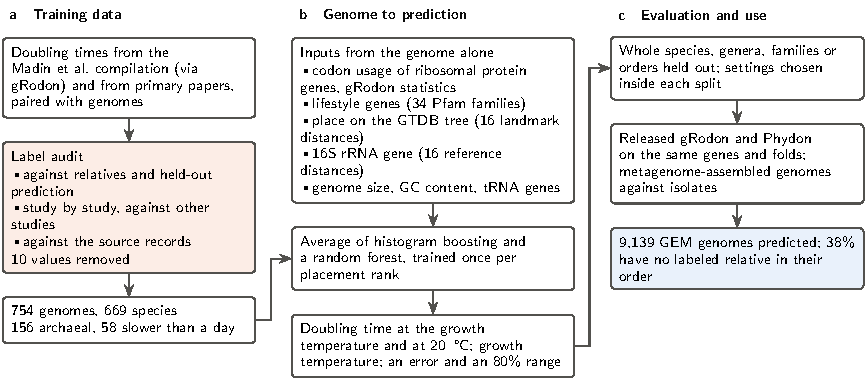
\includegraphics[width=0.82\textwidth,alt={Flow diagram in three columns. Training data: doubling times from the Madin compilation and primary papers, a label audit that removed values which are not maximal growth rates, and the final training set. Genome to prediction: inputs computed from the genome, a model averaging histogram boosting and a random forest, and three predicted quantities with errors and ranges. Evaluation and use: lineage-held-out evaluation, comparison with released tools and with metagenome-assembled genomes, and predictions for the GEM catalog.}]{fig1_overview_standalone}
\caption{Overview. (a) Growth rates were collected and audited for values that are not maximal growth rates. (b) Every input
is computed from the genome, so the same model applies to isolates and to metagenome-assembled genomes. (c) Accuracy is
measured with whole lineages held out, which is the situation of most environmental genomes, and the measured error at each
level of novelty is attached to every prediction.}
\label{fig:overview}
\end{figure*}


\begin{table}[t]\centering\footnotesize\setlength{\tabcolsep}{3pt}
\caption{Training data after the label audit. Rows are genomes with a measured doubling time; slow means a doubling time above 24 h; gene features are available where the genes could be predicted and annotated. The audit removed 10 values (Supplementary Table~\ref{S-tab:exclusions}). Genome size, GC content and tRNA count are computed from the genome, except in the rows marked $^{a}$, which take them from the compilation.}\label{tab:data}
\begin{tabular}{lrrrrr}
\toprule
Source & Genomes & Species & Archaea & Slow & Gene features \\
\midrule
gRodon's growth table & 294 & 209 & 0 & 14 & 294 \\
Madin et al., with traits$^{a}$ & 291 & 291 & 99 & 18 & 279 \\
Madin et al., genome only & 161 & 161 & 53 & 20 & 161 \\
Literature strains & 8 & 8 & 4 & 6 & 8 \\
\midrule
Total & 754 & 669 & 156 & 58 & 742 \\
\bottomrule
\end{tabular}
\end{table}


\subsection{One study was enough to create a biological effect}
After the audit, the training set holds \NGenomes genomes from \NSpecies species; \NArchaea are archaeal and \NSlow double
less than once a day (Table~\ref{tab:data}). We removed \NExcluded values from \NExcludedSourcesWord sources, each only after a
second source for the species, or the study itself, showed that it was not a maximal growth rate at the stated temperature
(Supplementary Table~\ref{S-tab:exclusions}).

The case that shaped the audit involved \NExcludedKevbrinaWord methanotrophs. The compilation gives them doubling times of
\KevLabelMin to \KevLabelMax hours, taken from a study of growth at low temperature \citep{kevbrina2001}. The records of the
same study in the source compilation say \KevRecordMin to \KevRecordMax hours, about \KevRatio times more, which points to a
unit slip somewhere between the two. Neither version is a maximal growth rate. Yet with relatedness controlled, these
\NExcludedKevbrinaWord values alone make carriers of methane or ammonia monooxygenase look \KevFoldWith-fold slower (95\%
interval \KevLowWith to \KevHighWith, adjusted $p=\KevPWith$), exactly the kind of effect one would cite as evidence that
organisms on thin energy budgets grow slowly. Without them the estimate is \KevFoldWithout-fold (\KevLowWithout to
\KevHighWithout, adjusted $p=\KevPWithout$). Because the four values came from one study and agreed with each other, every
methanotroph genus looked slow, and no comparison with relatives could have caught it.

That is why the audit compares each study with evidence from other studies. With the exclusions switched off, the
study-level check recovers \PosCtrlCaughtWord of the \PosCtrlNWord values we had removed before it existed. The one it misses,
a lag-phase measurement of \textit{Klebsiella oxytoca}, is the only value from its study and was caught by the comparison with
relatives instead. On the current labels the check flags \NStudiesFlagged of \NStudiesCompared studies, and we found a
plausible reason for each when we read them, such as rich-medium rates of haloarchaea at their optimum. Most studies contribute
a single value, so the audit lowers the error rate of the labels but cannot certify them.

\begin{figure*}[t]
\centering
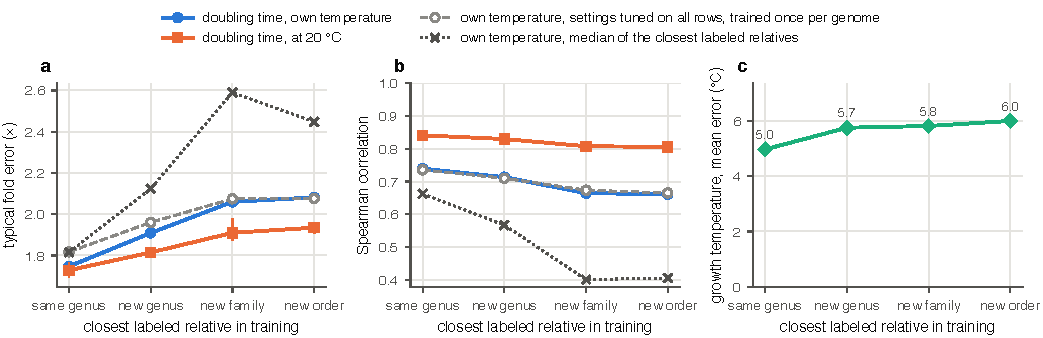
\includegraphics[width=\textwidth,alt={Three line panels against the closest labeled relative (same genus, new genus, new family, new order). Panel a: typical fold error of the doubling time rises with novelty and is lower for the 20 C value; the median of the closest labeled relatives is close to the model with species held out and clearly worse with families or orders held out. Panel b: Spearman correlation falls with novelty. Panel c: mean absolute error of growth temperature rises slightly with novelty.}]{fig2_accuracy}
\caption{Accuracy by the closest labeled relative of a genome, with that whole level held out (settings chosen inside each
split, \NSeedsHeadline seeds; bars span the seeds). (a) Typical fold error of the doubling time at the growth temperature and
at \TRefC\,\textdegree C. The dashed line is the same model with settings chosen on all labeled genomes and each genome
trained once, the scheme behind the error table released with the predictions; the dotted line predicts each genome by
the median label of its closest labeled relatives. (b) Spearman correlation. (c) Mean absolute error
of the growth temperature.}
\label{fig:accuracy}
\end{figure*}

\subsection{Accuracy falls with lineage novelty, and each prediction can carry its error}
We held out whole species groups, genera, families or orders, so that every test genome has its closest labeled relative at
a known level, and chose the model settings inside each split (Figure~\ref{fig:accuracy}, Supplementary
Table~\ref{S-tab:accuracy}). With a relative in the same genus, the predicted doubling time is typically off by
\ErrSameGenus-fold (95\% interval \CIErrLoSameGenus to \CIErrHiSameGenus; Spearman \RhoSameGenus). With the whole order held
out it is off by \ErrNewOrder-fold (\CIErrLoNewOrder to \CIErrHiNewOrder; Spearman \RhoNewOrder). Most of the loss happens
before the family level. The doubling time at \TRefC\,\textdegree C is predicted better at every level (\ErrRefSameGenus- to
\ErrRefNewOrder-fold), because much of the spread in doubling times comes from temperature, which the model itself predicts to
within \TempMAESameGenus to \TempMAENewOrder\,\textdegree C on average.

\paragraph{Against taxonomy alone.} A simple alternative predicts each genome by the median label of its closest labeled
relatives. When only the species is held out, this is nearly as good as the model (\BaseRelErrSameGenus-fold; the interval of
the difference, \CIDiffLoSameGenus to \CIDiffHiSameGenus, includes zero), although it ranks genomes worse (Spearman
\BaseRelRhoSameGenus against \RhoSameGenus). As relatives become distant it falls well behind: \BaseRelErrNewFamily- and
\BaseRelErrNewOrder-fold with families or orders held out, against \ErrNewFamily- and \ErrNewOrder-fold for the model.
Trained on labels shuffled across genomes, the model is no better than the median (\ShuffleErrSpecies-fold, Spearman
\ShuffleRhoSpecies), so the evaluation itself creates no accuracy.

\paragraph{Robustness.} Three further checks, run with the deployed settings over \TenNSeeds splits, leave these conclusions
intact (Supplementary Table~\ref{S-tab:robust}). Once the genus is held out, the model beats the relatives' median in
\TenModelWinsDeepMin of \TenNSeeds splits at every level (per genome $p$ \TenPGenomeDeepMax); with only the species held out
the two stay close (\TenModelErrSpecies- against \TenBaseErrSpecies-fold) and the model still ranks better. One input,
gRodon's own estimate, comes from a regression whose coefficients saw our species; refitting that regression inside each
split raises the error by at most \RefitMaxDiff, which bounds any leakage through it. Dropping the \FlagNLabels labels from
studies that the audit flagged but kept lowers the error on the remaining genomes slightly (\FlagErrOrder- against
\FlagFullErrOrder-fold with orders held out).

\paragraph{Training scheme.} Entering each training genome once for each of its four tree placements lowers the error with
the species held out from \FixedErrSameGenus- to \CoarseErrSameGenus-fold. Choosing the settings inside each split changes
the error at the growth temperature by at most \SelectMaxDiff, but at \TRefC\,\textdegree C it is slightly worse with orders held out
(\ErrRefNewOrder- against \FixedErrRefNewOrder-fold), so the released \TRefC\,\textdegree C errors are slightly optimistic.

\paragraph{Slow growers and archaea.} Slow growth is ranked better than it is predicted. The area under the curve for a
doubling time above a day is \AucSameGenus with the species held out and \AucNewOrder with orders held out, but predictions
are pulled toward the middle of the range. With the species held out, only \SlowCalledSpecies of \SlowTotalSpecies slow
species groups get a prediction above a day (\SlowCalledTrueSpecies correctly); with orders held out the count drops to \SlowCalledOrder. The typical
error of slow growers is \ErrSlowSpecies- to \ErrSlowOrder-fold, almost always toward faster growth. A prediction above a day
is therefore strong evidence of slow growth, while a short one is weak evidence against it. Archaea are also predicted less
well than bacteria (\ErrArchOrder- against \ErrBactOrder-fold with orders held out).

\paragraph{Ranges and the probability of slow growth.} Ranges set by novelty level alone contain \CovNovAllSpecies\% of
measured values with species held out and \CovNovAllOrder\% with orders held out, but only \CovNovArchOrder\% for archaea from held-out
orders. Setting them by novelty level and domain restores at least \CovDomArchMin\% for archaea, and these are the ranges we
release. No range built from the inputs can hold for organisms that are slow in truth (\CovDomSlowMin\% to
\CovDomSlowMax\%), since the model cannot single them out. For that question we release a probability of growing slower than
a day. It ranks genomes well (AUC \SlowProbAucSpecies and \SlowProbAucOrder) and is calibrated (error at most
\SlowProbECEMax), but it is modest: in the fifth of genomes with the highest probability, \SlowProbTopSpecies\% are slow,
against \SlowBaseRate\% overall.

\begin{table}[t]\centering\footnotesize\setlength{\tabcolsep}{3pt}
\caption{The released gRodon and Phydon against this model on the same 680 genomes, genes and species-held-out folds (mean of 3 seeds; this model built inside each split as in Algorithm~\ref{alg:nested}). T: the measured growth temperature is given as an input. Error: typical fold error; $\rho$: Spearman correlation; AUC: for a doubling time above a day. Wins: genomes, of those both methods predict, for which this model (without or with the temperature) has the smaller absolute log error, averaged over seeds, with the paired Wilcoxon $p$. Phydon placed 665 genomes.}\label{tab:released}
\begin{tabular}{@{}lccccc@{\hspace{4pt}}c@{}}
\toprule
& & & & & \multicolumn{2}{c}{Wins of this model} \\
\cmidrule(lr){6-7}
Method & T & Error & $\rho$ & AUC & without T & with T \\
\midrule
This model & no & 1.76 & 0.72 & 0.85 & -- & -- \\
This model & yes & 1.70 & 0.76 & 0.87 & -- & -- \\
gRodon & no & 2.40 & 0.52 & 0.75 & 424/680 ($<$0.001) & 453/680 ($<$0.001) \\
gRodon & yes & 1.92 & 0.73 & 0.84 & 349/680 (0.07) & 383/680 ($<$0.001) \\
Phydon & yes & 1.85 & 0.70 & 0.81 & 347/665 (0.11) & 355/665 ($<$0.001) \\
\bottomrule
\end{tabular}
\end{table}


\subsection{Against gRodon and Phydon, the model helps most when the temperature is unknown}
We ran the released gRodon \citep{weissman2021} and Phydon \citep{xu2025} on the same \RelN genomes, genes and
species-held-out folds as our model, after removing each fold's test species from Phydon's own training table (Methods). Both
tools need the measured growth temperature. Given it too, our model has a typical error of \RelOursTempErr-fold, against
\RelGRodonErr-fold for gRodon and \RelPhydonErr-fold for Phydon (Table~\ref{tab:released}), with a higher Spearman correlation
and area under the curve. It is better in every seed and, per genome, against both tools ($p=$\,\PairTempGRodonP and
\PairTempPhydonP).

An uncultured genome comes without a temperature, and without it gRodon's error rises to \RelGRodonNoTempErr-fold. Our model,
which predicts the temperature itself, keeps an error of \RelOursErr-fold. That is lower than either tool's error with the
temperature, in every seed, but per genome the difference is not significant (\PairGRodonBetter of \PairGRodonN genomes
favour our model against gRodon, $p=\PairGRodonP$; \PairPhydonBetter of \PairPhydonN against Phydon, $p=\PairPhydonP$).
Without the temperature, then, the model matches the released tools given it rather than beating them. The tools keep one
further advantage in this comparison: their parameters were fitted on data that include our test species.

With whole orders held out (and cut from Phydon's training table), Phydon's error rises to \RelOrdPhydonErr-fold, while
gRodon, which uses no relatives, stays at \RelOrdGRodonErr-fold given the temperature. Our model then ties with gRodon given
the temperature (\RelOrdOursTempErr-fold, $p=\PairOrdTempGRodonP$) and trails it without (\RelOrdOursErr-fold,
$p=\PairOrdGRodonP$), but stays ahead of gRodon without the temperature (\RelOrdGRodonNoTempErr-fold,
$p$\,\PairOrdGRodonNoTempP), the case of an uncultured genome.

\subsection{On species outside both training compilations}
To test the released model on labels it had never seen, we collected \ExtNCurated doubling times from species descriptions,
each the fastest growth in pure culture, for species absent from the compilation of \citet{madin2020} (by NCBI taxonomy
identifier, which survives renaming) and from our labels, with no training genome in their GTDB species (Methods;
Supplementary Table~\ref{S-tab:external}). \ExtN have usable genomes, \ExtNNewOrder without a labeled relative in their
order. The model is off by \ExtModelErr-fold (95\% interval over genera \ExtModelLo to \ExtModelHi, Spearman \ExtModelRho),
against \ExtBaseErr-fold for the relatives' median and \ExtGRodonErr-fold for gRodon without a temperature, and is closer for
\ExtBetterBase and \ExtBetterGRodon of the \ExtN species ($p=\ExtPBase$ and \ExtPGRodon). The error grows from
\ExtModelErrSameGenus-fold within a labeled genus to \ExtModelErrNewOrder-fold in a new order, more than in
cross-validation. The ranges are too narrow here, holding \ExtCoverage\% of the values instead of 80\% ($p=\ExtCoverageP$)
and \ExtCoverageSlowIn of the \ExtNSlow species slower than a day; the slow-growth probability ranks those \ExtNSlow well
(AUC \ExtSlowAuc), but none is predicted to take more than a day.

\subsection{What the accuracy comes from}
\begin{table*}[t]\centering\footnotesize\setlength{\tabcolsep}{3.5pt}
\caption{What each part contributes. Each row changes one thing in the final model and gives the mean change over 10 seeds, with the number of seeds in which the variant did better in brackets; $^{*}$ paired Wilcoxon $p<0.05$. Typical error is the fold error of the median genome (lower is better); AUC ranks genomes slower than a day. All variants are scored on the same genomes and folds, with the deployed settings and each genome entered once. The seeds reshuffle the same genomes, so $p$ measures how consistent a change is across splits, not independent replication. $^{\dagger}$The earlier learner (gradient boosting, 200 trees of depth 3) against the tuned average, both with settings chosen inside each split (5 seeds).}\label{tab:ablations}
\begin{tabular}{lcccccc}
\toprule
& \multicolumn{3}{c}{Species held out} & \multicolumn{3}{c}{Orders held out} \\
\cmidrule(lr){2-4} \cmidrule(lr){5-7}
& Typical error ($\times$) & Spearman & AUC, slow & Typical error ($\times$) & Spearman & AUC, slow \\
\midrule
final model & 1.819 & 0.740 & 0.838 & 2.093 & 0.654 & 0.803 \\
\midrule
without gRodon statistics & +0.110$^{*}$ (0/10) & $-$0.044$^{*}$ (0/10) & $-$0.010$^{*}$ (0/10) & +0.295$^{*}$ (0/10) & $-$0.080$^{*}$ (0/10) & $-$0.045$^{*}$ (0/10) \\
without lifestyle genes & +0.005 (4/10) & $-$0.002$^{*}$ (1/10) & 0.000 (3/10) & $-$0.020 (6/10) & +0.005$^{*}$ (8/10) & +0.002$^{*}$ (7/10) \\
without any gene features & +0.274$^{*}$ (0/10) & $-$0.078$^{*}$ (0/10) & $-$0.033$^{*}$ (0/10) & +0.551$^{*}$ (0/10) & $-$0.195$^{*}$ (0/10) & $-$0.076$^{*}$ (0/10) \\
without 16S & $-$0.002 (7/10) & +0.002$^{*}$ (8/10) & 0.000 (6/10) & 0.000 (6/10) & 0.000 (7/10) & $-$0.010$^{*}$ (1/10) \\
without GTDB phylogeny & +0.026$^{*}$ (1/10) & $-$0.008$^{*}$ (0/10) & +0.002 (7/10) & $-$0.023$^{*}$ (8/10) & +0.002 (7/10) & +0.006$^{*}$ (10/10) \\
without the added species & +0.040$^{*}$ (0/10) & $-$0.009$^{*}$ (0/10) & $-$0.003$^{*}$ (1/10) & +0.040$^{*}$ (0/10) & $-$0.004 (3/10) & $-$0.006$^{*}$ (2/10) \\
with energy-metabolism genes & +0.002 (4/10) & 0.000 (5/10) & +0.001 (7/10) & +0.013$^{*}$ (3/10) & $-$0.001 (4/10) & $-$0.001 (4/10) \\
with predicted growth temperature & $-$0.015 (6/10) & $-$0.001 (4/10) & 0.000 (5/10) & $-$0.015$^{*}$ (8/10) & +0.004$^{*}$ (8/10) & +0.002 (7/10) \\
earlier learner, nested$^{\dagger}$ & & & & +0.015 (1/5) & $-$0.021 (0/5) & $-$0.012 (0/5) \\
\bottomrule
\end{tabular}
\end{table*}


The accuracy comes from the genes (Table~\ref{tab:ablations}; deployed settings, one placement per genome). Without gRodon's
codon usage statistics the error rises from \AblFinalErrSpecies- to \AblGStatErrSpecies-fold with the species held out and
from \AblFinalErrOrder- to \AblGStatErrOrder-fold with orders held out; without any gene features it rises to
\AblGenesErrSpecies- and \AblGenesErrOrder-fold, worse in all \NSeedsAblation seeds. The species we added to the earlier
training data help at both levels. The GTDB phylogeny helps only when a relative in the same genus is labeled, as one would
expect when the closest relatives are far away. The 16S inputs leave the typical error unchanged; with orders held out they
add a little to the ranking of slow growers (AUC \AblFinalAucOrder against \AblSixteenAucOrder without them). Energy-metabolism genes do not help, and a predicted growth temperature as an extra input gains too
little to justify a second model. The tuned average of two learners improved only slightly on the earlier single model
(\TuneErrBefore- to \TuneErrAfter-fold with orders held out).

\paragraph{A learned representation.} A generic protein language model does as well as our hand-built features. A ridge
probe on ESM-2 embeddings \citep{lin2023} of each genome's ribosomal proteins and \EsmNOther other proteins reaches
\EsmProbeErrSameGenus-fold with species held out and \EsmProbeErrNewOrder-fold with orders held out, against
\EsmFeatErrSameGenus- and \EsmFeatErrNewOrder-fold for the features (per genome $p=\EsmProbePSameGenus$ and
\EsmProbePNewOrder). The two are complementary: adding \EsmPCComb principal components of the embeddings to the features
lowers the error to \EsmCombErrSameGenus- and \EsmCombErrNewOrder-fold ($p=$\,\EsmCombPSameGenus and \EsmCombPNewOrder;
Supplementary Table~\ref{S-tab:esm}). The released predictions do not use embeddings yet.

\paragraph{A trap in the 16S input.} Most labeled species first had their 16S gene retrieved from NCBI by name, while a GEM
genome's gene is cut from the genome itself; for \SixteenFarther labeled genomes the NCBI copy was farther from the
genome's own gene than from another species. A model trained on NCBI copies and given genome copies, as the GEM genomes had
been, did worse in every seed (\SixteenErrMixedOrder- against \SixteenErrNcbiOrder-fold with orders held out). All results
here use the copy cut from the genome wherever barrnap finds one (\SixteenNGenomeCopy genomes).

\begin{figure*}[t]
\centering
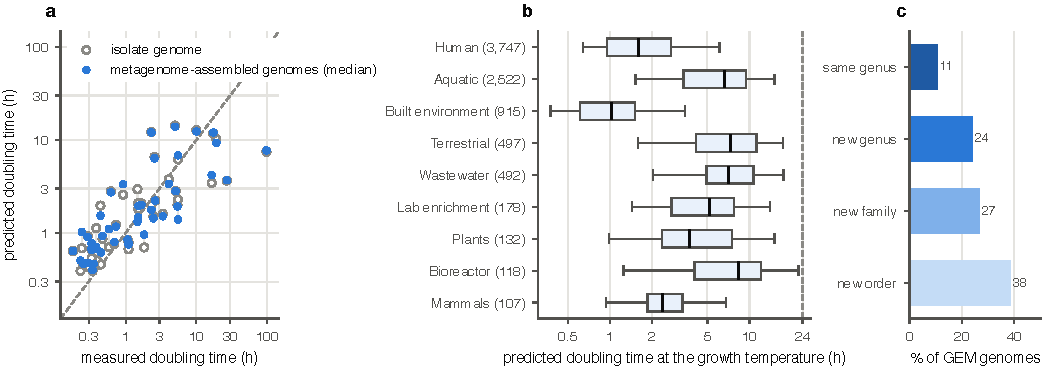
\includegraphics[width=\textwidth,alt={Panel a: scatter of predicted against measured doubling time, with isolate and metagenome-assembled predictions for each species joined by lines, lying close together. Panel b: box plots of predicted doubling time of GEM genomes by habitat. Panel c: bar chart of the share of GEM genomes by closest labeled relative.}]{fig4_mags_gem}
\caption{From isolates to the GEM catalog. (a) Predicted against measured doubling time for \MagNSpecies species held out of
training, predicted from the isolate genome (open) and from the species' metagenome-assembled genomes in GEM (filled, median
over the assembled genomes of a species); lines join the two predictions. (b) Predicted doubling times of GEM genomes by
habitat, for habitats with at least 100 genomes (boxes: quartiles; whiskers: 5th and 95th percentiles; dashed line: one day).
(c) Closest labeled relative of the GEM genomes.}
\label{fig:mags}
\end{figure*}

\subsection{Predictions transfer to metagenome-assembled genomes}
The GEM catalog contains \MagNGenomes assembled genomes of \MagNSpecies species with a measured growth rate. With each species
held out of training, predictions from its assembled genomes are off by \MagErr-fold (95\% interval \CIMagErrLo to
\CIMagErrHi), against \MagIsoErr-fold from its isolate genome; the interval of the difference (\CIMagDiffLo to \CIMagDiffHi)
includes zero (Figure~\ref{fig:mags}a). The two predictions sit close together, a median of \MagGap-fold apart, and for
\MagGapSmaller of the \MagNSpecies species the gap is smaller than the error of the isolate prediction itself. Most of the
error on assembled genomes is the error the model makes on any new species, not a cost of assembly.

\begin{figure}[t]
\centering
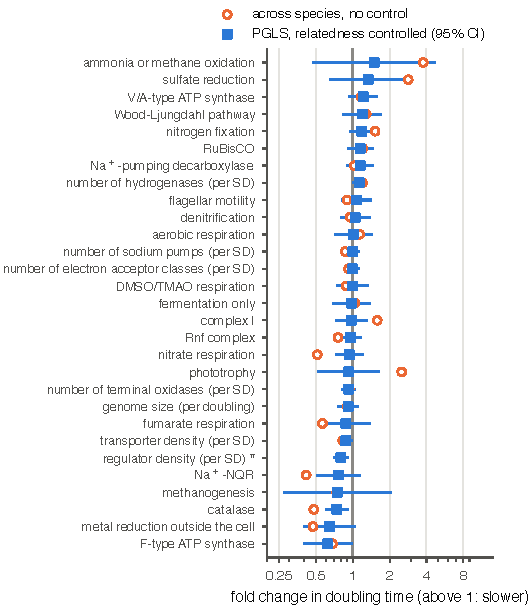
\includegraphics[width=\columnwidth,alt={Forest plot of fold change in doubling time for each gene-content input, without and with phylogenetic control; with control, most intervals cross one and no energy-metabolism input remains significant after adjustment for the number of inputs.}]{fig5_lifestyle}
\caption{Gene content and doubling time across \PglsNGroups species groups, without control for relatedness (open circles)
and with phylogenetic generalized least squares (squares, 95\% intervals), with growth temperature and domain as
covariates. Effects are fold changes for carrying a gene, per standard deviation of a count or density, or per doubling of
genome size. $^{*}$Adjusted $p<0.05$.}
\label{fig:lifestyle}
\end{figure}

\subsection{Slow growers carry fewer transporter genes, not an energy-poor metabolism}
Doubling time is strongly patterned by relatedness (Pagel's $\lambda=\PglsLambda$ over \PglsNGroups species groups), so a raw
comparison across species counts one slow clade many times over. Across species, several energy-related inputs do look
associated with growth rate: phototrophy, sulfate reduction and monooxygenases with slower growth, nitrate respiration and the
Na$^+$-translocating NADH dehydrogenase with faster growth (Figure~\ref{fig:lifestyle}). Once relatedness is controlled, none
of the inputs that describe how an organism makes energy is associated with its doubling time (adjusted $p\ge\PglsEnergyMinP$
for all of them).

Two inputs about how an organism senses and draws on its surroundings remain. A higher density of regulator genes goes with
faster growth (\PglsRegFold-fold per standard deviation, adjusted $p=\PglsRegP$), but the association rests on the
Pseudomonadota and disappears without them. The clearest signal for growing slower than a day is a low density of transporter
genes: the odds of being slow fall to \SlowTransporterOR per standard deviation more transporters ($p=$\,\SlowTransporterP),
with \KEigen phylogenetic eigenvectors as covariates, and the result holds with half or one and a half times as many.

\subsection{Growth rates for the GEM catalog}
Across the \NGEMPredicted high-quality GEM genomes, the median predicted doubling time at the growth temperature is
\GEMMedianHours hours (Figure~\ref{fig:mags}b). Only \GEMNSlow genomes (\GEMShareSlow\%) are predicted to double less than
once a day, most of them \GEMSlowTopOrder (\GEMSlowTopOrderN) and ammonia-oxidizing archaea of the \GEMSlowSecondOrder
(\GEMSlowSecondOrderN). Genomes from the human body (median \GEMMedianHuman hours, \GEMNHuman genomes) and the built
environment (\GEMMedianBuilt hours) are predicted to grow faster than those from aquatic (\GEMMedianAquatic hours) and
terrestrial habitats (\GEMMedianTerrestrial hours). The habitats also differ in how well labeled relatives cover them:
\GEMNewOrderHuman\% of human-associated genomes have no labeled relative in their order, against \GEMNewOrderAquatic\% of
aquatic and \GEMNewOrderTerrestrial\% of terrestrial ones (Figure~\ref{fig:mags}c). Predictions for environmental habitats
therefore carry the larger errors of Figure~\ref{fig:accuracy}, and each is released with its novelty level, error and range.

\section{Discussion}
\paragraph{Where the model earns its keep.} When a relative in the same genus has a measured growth rate, simply taking the
median of the relatives gets close to the model, which then adds mostly a better ranking. The model pulls ahead as the
relatives get further away, and that is where most environmental genomes sit: \GEMShareNoGenus\% of the high-quality GEM
genomes have no labeled relative in their genus and \GEMShareNewOrder\% none in their order. In that regime the accuracy comes
from the genes, through gRodon's codon statistics and the gene features, while the tree position and the 16S gene add
little. We would use the predictions to compare and rank genomes rather than to quote a single doubling time, and for
comparisons across habitats we would use the doubling time at \TRefC\,\textdegree C, which removes the part of the difference
that temperature explains. Slow growth remains the weak point. Slow growers are ranked well but rarely predicted above a day,
so the \GEMNSlow slow GEM genomes are a short list rather than a count, and the slow-growth probability is the better guide.
The clearest next gain is to add protein language-model embeddings to the features.

\paragraph{Labels and inputs.} The \NExcludedKevbrinaWord values from a single study were enough to produce a \KevFoldWith-fold effect, significant
with relatedness controlled, that would have read as support for an attractive biological idea. The values agreed with each
other, so no comparison with relatives could have flagged them; only tracing them back to their source did. We would check
values from studies that contribute several species, or that differ from their source record, before using them. The 16S
result is the same trap on the input side: copies retrieved by name and copies cut from the genome were similar enough to pass
our drift check and different enough to cost accuracy. Finally, the measured temperature lowers gRodon's error from
\RelGRodonNoTempErr- to \RelGRodonErr-fold, an advantage an uncultured genome does not have. Predictors meant
for metagenome-assembled genomes should be judged without it, and with whole lineages held out.

\paragraph{Slow growth and energy.} Organisms in energy-poor environments are often thought to grow slowly because their
energy supply is thin \citep{hoehler2013,lever2015}. Across species, several energy-related genes do track doubling time, but
none survives control for relatedness and for the number of inputs tested, in the main analysis or in the three checks of
Supplementary Table~\ref{S-tab:pgls}. These associations follow the tree. What remains is that slow growers carry fewer
transporter genes, in line with what is known about oligotrophic and copiotrophic marine bacteria \citep{lauro2009}. Our
labeled organisms all grow in culture and few live on the thinnest energy budgets, so this argues against the simplest form
of the low-energy explanation among cultured organisms, not against it in general.

\paragraph{Limitations.} The labels are maximal rates in culture, which can be far above rates in the environment
\citep{gibson2018,brown2016}. The training set is small (\NGenomes genomes, \NSlow slower than a day), and predictions shrink
toward the middle of the range. Some labels are surely still wrong after the audit. The GEM taxonomy comes from an older GTDB
release, so the novelty levels we report are worst cases. On species outside both compilations the ranges held fewer values
than they should, and missed most slow growers, so for a new lineage the true uncertainty is larger than the range suggests. In our tests, adding labeled species helped more than changing the learner, so new growth measurements for lineages
without cultured members would probably improve the predictions most.


\bibliographystyle{gem-oup}
\bibliography{refs}
\end{document}
